\documentclass[a4paper,11pt]{report}
\usepackage[utf8]{inputenc}  
\usepackage[italian]{babel}
\usepackage{indentfirst}
\usepackage{tocloft}
\renewcommand{\cftchapdotsep}{\cftdotsep}
\raggedbottom
\usepackage{epigraph}
\usepackage[T1]{fontenc}        % include i font in maniera vettoriale azichè 
\usepackage{lmodern}            % latin modern fonts
\usepackage{graphicx,color}     % per le immagini
\usepackage{latexsym}           
\usepackage{setspace}          
\usepackage{amsmath}            % package per la matematica
\usepackage{amsfonts}           % idem
\usepackage{amssymb}            % idem
\usepackage{amsthm}             % idem
\usepackage{fancyvrb}           % package per il comando VerbatimInput
\usepackage{hyperref}
\usepackage{listings}
\usepackage{lettrine}

\lstset{language = Java, numbers = left, basicstyle=\footnotesize, numberstyle=\footnotesize}

%Da sistemare con l'icona del programma.
\title{\textbf{Progetto \newline Laboratorio Programmazione di rete \newline Mini-KaZaA}}
\author{Andrea Di Grazia, Massimiliano Giovine
                }
\date{Anno Accademico 2008 - 2009}

\begin{document}
\maketitle
\tableofcontents

%Introduzione al progetto
\chapter{Introduzione}
\section{Una panoramica generale.}
Il progetto Mini-KaZaA mira allo sviluppo di un sistema p2p per lo scambio di file su WAN, ispirato alla più famosa
rete p2p KaZaA.
Ogni peer\footnote{Ogni nodo della rete è un pari all'interno del network poichè funziona sia da client, per ciò che concerne la ricerca e il download dei file, sia da server per la condivisione dei file o lo smistamento delle ricerche nella rete p2p.} partecipante alla rete Mini-KaZaA condivide un insieme di files con gli altri peer connessi e può ricercare file all'interno della rete e effettuarne il download.

Mini-KaZaA prevede due tipi diversi di peer:
\begin{itemize}
 \item \textbf{Super Nodes (SN): }i SN hanno il compito di gestire le comunicazioni all'interno della rete;
 \item \textbf{Ordinary Nodes (ON): }gli ON hanno responsabilità più limitate, condividono e cercano file nella rete.
\end{itemize}

Nella rete Mini-KaZaA è prevista anche un'altra entità chiamata \textbf{Bootstrap Servers} che contiene la lista di tutti i peer connessi alla rete e dalla quale ogni nodo che desidera entrare a far parte della rete può scaricare la lista aggiornata di tutti i SN presenti.

La rete si costruisce automaticamente dai vari peer secondo un preciso schema e si mantine stabile grazie a processi automatizzati che lavorano in background, completamente trasparenti all'utente.

\section{La rete Mini-KaZaA.}
Ogni peer della rete Mini-KaZaA viene configurato esplicitamente dall'utente al primo avvio come SN o come ON. Successivamente non sarà possibile cambiare tale configurazione.

Al momento della connessione alla rete ogni peer, SN o ON, contatta un Bootstrap server che gli fornisce la lista aggiornata di SN presenti in quel momento all'interno della rete.

Un ON sceglie il migliore SN per lui e si connette ad esso. Un SN mantiene in memoria la lista di riferimenti a SN che gli servirà, in un secondo momento, per smistare le interrogazioni. Gli SN, inoltre, avendo un sistema dinamico di connessione ai pari SN esplorano a ogni interrogazione porzioni nuove della rete in modo tale che vi siano il meno possibile porzioni isolate della rete.

%Spiegazione implementazione del bootstrap server
\chapter{Bootstrap Server}

\section{Il Bootstrap server in generale}
Il Bootstrap server ha il compito di tenere un indice di tutti i SN presenti nella rete che abbiano
una certa affidabilità. 
Per poter fare questo fornisce un servizio di RMI\footnote{Remote Method Invocation, tramite questo servizio è possibile invocare metodi che si trovano su una macchina diversa da quella in cui si trova la chiamata a procedura.} tramite il quale i SN si possono iscrivere alla rete Mini-KaZaA e richiedere liste aggiornate.

Gli aggiornamenti vengono spediti a ogni SN presente nella lista del Bootstrap server tramite un sistema di \emph{callbacks}\footnote{Ogni nodo mette a disposizione del Bootstrap server alcune chiamate di procedura che, richiamate, consentono di inviare aggiornamenti.}

Il Bootstrap server deve fornire questo servizio anche agli ON che vogliono entrare nella rete per poter individuare il ``miglior''\footnote{Spiegeremo nella sezione \ref{sec:scelta_sn} i parametri secondo i quali ogni ON sceglie un SN al quale connettersi.} SN al quale potersi connettere.
Per questa ragione si è reso necessario indicizzare anche gli ordinary node all'interno del bootstrap server.

\section{Entriamo nel dettaglio}
Il bootstrap server si avvia dal main situato all'interno del file \verb|BootstrapService.java| e subito crea il servizio RMI sulla porta 2008 da mettere a disposizione per i vari nodi della rete con le seguenti istruzioni:
\newline
\begin{lstlisting}
Registry registry = LocateRegistry.createRegistry(2008);
BootStrapServer bss = new BootStrapServer(g,sn_list);

BootStrapServerInterface stub = 
	(BootStrapServerInterface) 
	UnicastRemoteObject.exportObject(bss, 2008);


SupernodeCallbacksImpl client_impl = 
	new SupernodeCallbacksImpl(
	new SupernodeList(), 
	new NodeConfig());
            
SupernodeCallbacksInterface client_stub = 
	(SupernodeCallbacksInterface) 
	UnicastRemoteObject.exportObject( client_impl,2008);
\end{lstlisting}

Con le prime istruzioni il Bootstrap server mette a disposizione tutti i metodi della classe \verb|BootStrapServerInterface| che sono i seguenti:
\newline
\begin{lstlisting}
public boolean 
	addSuperNode(NodeInfo new_node) throws RemoteException;

public boolean 
	removeSuperNode(NodeInfo new_node) throws RemoteException;

public boolean 
	addOrdinaryNode(NodeInfo new_node) throws RemoteException;

public boolean 
	removeOrdinaryNode(NodeInfo new_node) throws RemoteException;

public ArrayList<NodeInfo> 
	getSuperNodeList() throws RemoteException;
\end{lstlisting}

Con le istruzioni alla riga 9 e 14 registra l'interfaccia di callback, definita nel package del Super Node,  \verb|SupernodeCallbacksInterface| che ha i seguenti metodi:
\newline
\begin{lstlisting}
public void 
	notifyMeAdd(NodeInfo new_node) throws RemoteException;

public void 
	notifyMeRemove(NodeInfo new_node) throws RemoteException;
\end{lstlisting}

Per poter trasmettere e ricevere le informazioni riguardanti i vari nodi della rete, il client Mini-KaZaA e il Bootstrap server usano una classe serializzabile che si chiama \verb|NodeInfo| che analizzamo nella sezione \ref{sec:nodeinfo}

\section{La classe NodeInfo}\label{sec:nodeinfo}
La classe \verb|NodeInfo| si trova nel package \verb|lpr.minikazaa.bootstrap| ma viene utilizzata da tutto il pacchetto Mini-KaZaA per poter inviare nella rete le informazioni relative ai nodi.

Questa classe rappresenta le informazioni utili di un nodo con le sue variabili private.

\begin{lstlisting}
private InetAddress ia_node;
private int door;
private String id_node;
private String username;
private SupernodeCallbacksInterface stub;
private long ping;
private boolean is_sn;
\end{lstlisting} 

Le prime tre variabili private riguardano tutte le informazioni di rete dei nodi, ovvero l'indirizzo IP,
la porta di connessione e un id univoco ottenuto facendo la concatenazione della rappresentazione decimale
dell'indirizzo IP.

La variabile privata \verb|private SupernodeCallbacksInterface stub| rappresenta l'interfaccia per le callbacks che viene messa a disposizione dal nodo. In questo modo il bootstrap server può richiamare direttamente l'interfaccia delle callback di ogni nodo interessato all'aggionrnamento.

L'ultima variabile, \verb|private boolean is_sn| indica se il nodo al quale si riferiscono le informazioni, all'interno della rete ricopre il ruolo di SN o di ON.

La classe contiene tutti i metodi \verb|set| e \verb|get| per poter assegnare valori alle variabili private e per poterne ricavare il contenuto in qualsiasi momento.

\section{L'interfaccia grafica.}
L'interfaccia grafica fornisce le informazioni riguardo a ciò che avviene all'interno della rete.

\begin{figure}[t]
 \centering
 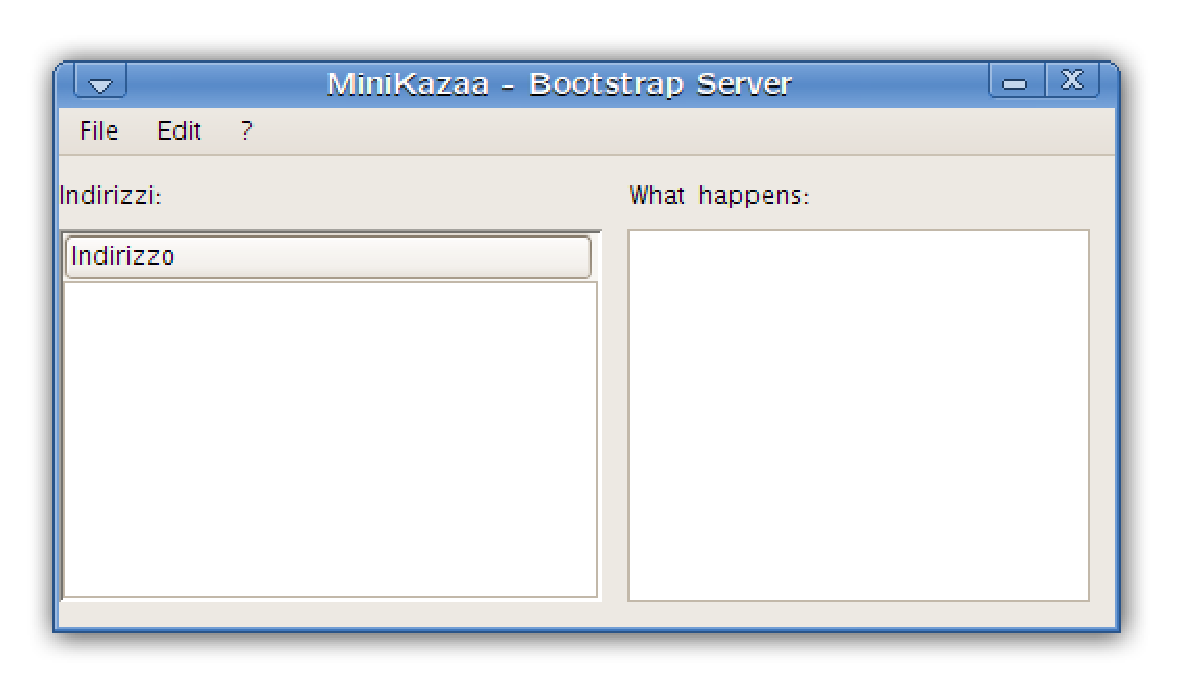
\includegraphics[width=300px,height=160px]{images/bss_grafica.eps}
 % bss_grafica.eps: 0x0 pixel, 300dpi, 0.00x0.00 cm, bb=14 14 564 329
 \caption{Interfaccia grafica del Bootstrap server}
 \label{fig:bss_grafica}
\end{figure}

Uno screenshot dell'interfaccia grafica principale del Bootstrap server si può vedere in Figura \ref{fig:bss_grafica}.

Nella parte a sinistra dell'interfaccia vengono inseriti gli \emph{id} di tutti i nodi che si connettono alla rete.

Nella parte destra, invece, vengono visualizzati dei messaggi che spiegano cosa avviene all'iterno della rete.




%Spiegazione implementazione del client della rete mini-kazaa
\chapter{Mini-KaZaA Client}
Oltre che di un Bootstrap server, la rete Mini-KaZaA si basa su un client che gli utenti possono usare per accedere alla rete e poter condividere e scaricare file.
\section{Mini-KaZaA Client in generale}
Mini-KaZaA client presenta tutte le funzionalità che consentono una condivisione peer to peer dei contenuti.
Ogni client al primo avvio chiede all'utente, tramite un comodo pannello, di scegliere il \emph{ruolo} da interpretare all'interno della rete.

Chi ha più risorse da mettere a disposizione e una banda di comunicazione più ampia può scegliere di essere un Super Node, che oltre a condividere e scaricare, ha la funzione di smistare le query nella rete e accettare richieste direttamente dagli Ordinary Node \emph{figli}. Chi ha meno risorse da mettere a disposizione può scegliere di essere un semplice Ordinary Node.

\section{Il codice di Mini-KaZaA client}
Il codice di Mini-KaZaA client è distribuito in tre diverse librerie:
\begin{itemize}
 \item \textbf{lpr.minikazaa.minikazaaclient}: questa libreria contiene classi comuni a tutti e due i tipi di client dal punto di vista logico. L'esempio più evidente è la classe \verb|MainGui.java|.
 \item \textbf{lpr.minikazaa.minikazaaclient.ordinarynode}: questa libreria contiene le classi che loogicamente appartengono al tipo di client Ordinary Node, ma che, all'occorrenza, possono essere importate anche da un Super Node.
 \item \textbf{lpr.minikazaa.minikazaaclent.supernode}: questa libreria, infine contiene tutte le classi che servono a un supernodo per funzionare e che appartengono a questo logicamente. Alcune di queste classi, come per esempio \verb|SupernodeCallbacksInterface.java|, vengono utilizzate anche dagli ORdinary Node.
\end{itemize}

Questa suddivisione è puramente logica visto che i due tipi di client differiscono solo per alcune caratteristiche.

Si è preferito dividere anche le classi che contengono gli stessi task per i SN e per gli ON per poter meglio gestire il codice e renderlo più modulare.
Un esempio è rappresentato dalle classi \verb|OrdinarynodeWorkingThread.java| e \verb|SupernodeWorkingThread.java| che hanno lo stesso compito, ma, che piuttosto che complicare con una serie di 
\begin{verbatim}
if <condizione> then 
	<blocco> 
else 
	<blocco>|
\end{verbatim}
si è preferito separare in due classi distinte.

Passiamo ora a una presentazione più particolareggiata del codice comune a Super Node e Ordinary Node.

\section{Le strutture dati comuni}
Per lo sviluppo di Mini-KaZaA è stato necessario predisporre una serie di strutture dati che tutto il software
utilizzi per condividere informazioni.

All'interno del package \verb|lpr.minikazaa.minikazaaclient| troviamo le seguenti classi che rappresentano strutture dati comuni a SN e ON:
\begin{itemize}
 \item \verb|NodeConfig.java|
 \item \verb|Query.java|
 \item \verb|Answer.java|
 \item \verb|SearchField.java|
 \item \verb|Download.java|
 \item \verb|DownloadRequest.java|
 \item \verb|DownloadResponse.java|
\end{itemize}

Guardiamo cosa si nasconde all'interno di ognuna di queste classi.

\subsection{NodeConfig.java}
La classe \verb|NodeConfig.java| contiene i seguenti attributi:
\newline
\begin{lstlisting}
private String user_name;
private int port;
private String bootstrap_address;
private int max_conn;
private int ttl;
private boolean is_sn;

//Calcolato all'avvio
private String my_address;
\end{lstlisting}

Questi attributi sono i campi che l'utente inserisce nel form al primo avvio del programma e contengono le informazioni di configurazione del nodo. 

\subsection{Query.java}
La classe \verb|Query.java| viene utilizzata dal client Mini-KaZaA per l'invio di richieste di file nella rete.

Contiene diversi attributi per i quali ci sono i metodi \verb|set| e \verb|get|. Questa classe inoltre implementa
le interfacce \verb|Serializable| e \verb|Cloneable|.
La prima serve per poter inviare su rete come flusso di byte l'oggetto \verb|Query|. La seconda invece serve per poter
copiare un'istanza dell'oggetto \verb|Query| in una seconda istanza.
\newline
\begin{lstlisting}
private String body_q;              //Regex of a sended query
private Answer body_a;              //Answer query
private OrdinarynodeFiles body_f;   //Notify a supernode to 
                                 	//have many files to share.
private NodeInfo id_origin;         //Source of a query
private NodeInfo sender;            //NodeInfo of sender node.
private NodeInfo receiver;          //NodeInfo of receiver node

private int ttl;                    //Time to live of a query
private int id;                     //Id of origin query
\end{lstlisting}

La classe \verb|Query| ha tre gruppi di attributi.Un primo gruppo descrive il contenuto della query e di conseguenza
il tipo di query. Un secondo gruppo serve per identificare i soggetti coinvolti nello scambio della query stessa.
Il terzo gruppo contiene invece parametri per l'identificazione della query. 

Analizziamo uno ad uno questi parametri per capire meglio come funzionano le query in Mini-KaZaA.
\begin{itemize}
 \item \verb|body_q|:
il vero corpo della query di richiesta di un file. \`{E} una stringa che contiene un
espressione regolare che il client Mini-KaZaA riesce a interpretare;

 \item \verb|body_a|:
la parte dell'oggetto \verb|Query| che contiene la risposta a una determinata richiesta. Analizzaremo la classe
\verb|Answer| successivamente;

 \item \verb|body_f|:
questo campo viene riempito da un ON che vuole inviare al proprio SN la sua lista di file per metterli a disposizione
di tutti;

 \item \verb|id_origin|:
per ogni query deve essere nota l'origine dalla quale proviene la query stessa per poi poterla correttamente fermare
al punto giusto e farla ritornare al mittente. Questo è il compito del campo \verb|id_origin|;

 \item \verb|sender|: 
questo campo indica uno dei due soggetti che sono impegnati in un singolo scambio di query, il nodo da cui parte;

 \item \verb|receiver|:
questo campo indica il nodo a cui deve arrivare la query in uno scambio;

 \item \verb|ttl|:
questo campo sta per \emph{Time To Live} e indica il numero di scambi per il quale la query deve continuare a esistere.
Serve principalmente per evitare che si creino dei cicli infiniti di scambio della query ottenendo quindi una valanga
di dati ridondanti con conseguente intasamento della rete;

 \item \verb|id|:
ogni nodo può inviare più query alla volta nella rete e il compito di questo campo è di identificare univocamente la
query presso il suo nodo origine.
\end{itemize}

\subsection{Answer.java}
La classe \verb|Answer.java| contiene i file che possono corrispondere ai criteri di una ricerca. 

\`{E} una classe molto semplice ma molto utile per indicizzare rapidamente i file.

Ecco il codice nel quale vengono dichiarati gli attributi della classe.
\newline
\begin{lstlisting}
//List of files that corresponding to a query.
private ArrayList <OrdinarynodeFiles> files;

//Id of origin query
private int id;
\end{lstlisting}

L'attributo \verb|files| è una lista di OrdinarynodeFiles, Sezione \ref{sec:on_files}.

La classe \verb|Answer.java| viene utilizzata 

L'attributo \verb|id| richiama semplicemente l'id univoco della query di cui fa parte l'oggetto \verb|Answer|.

\subsection{SearchField.java}
La classe \verb|SearchField.java| viene utilizzata dal client Mini-KaZaA per tenere in memoria tutti i risultati
associati a una richesta di file.
Da uno di questi campi poi vengono estratte le informazioni per eventuali download di file.

Anche questa classe è piuttosto semplice poichè funziona da appoggio alla rappresentazione grafica e per snellire
la quantità di informazioni da tenere in memoria per l'utente.

Il codice che descrive gli attributi della classe è il seguente:
\newline
\begin{lstlisting}
//File owner
private NodeInfo owner;

//File descriptor
private MKFileDescriptor file;
\end{lstlisting}

Con queste due semplici informazioni è possibile sia risalire al proprietario, compreso l'indirizzo ip da contattare
per il download, sia ottenere tutti i metadati del file da scaricare\footnote{I download così come le ricerche vengono
effettuati mediante l'hash univoco md5 che tratteremo nella Sezione \ref{sec:md5}}.

\subsection{Download.java}

\subsection{DownloadRequest.java}
\subsection{DownloadResponse.java}

\section{Il percorso di una query}
\section{La grafica del client Mini-KaZaA}
\begin{figure}[t]
 \centering
 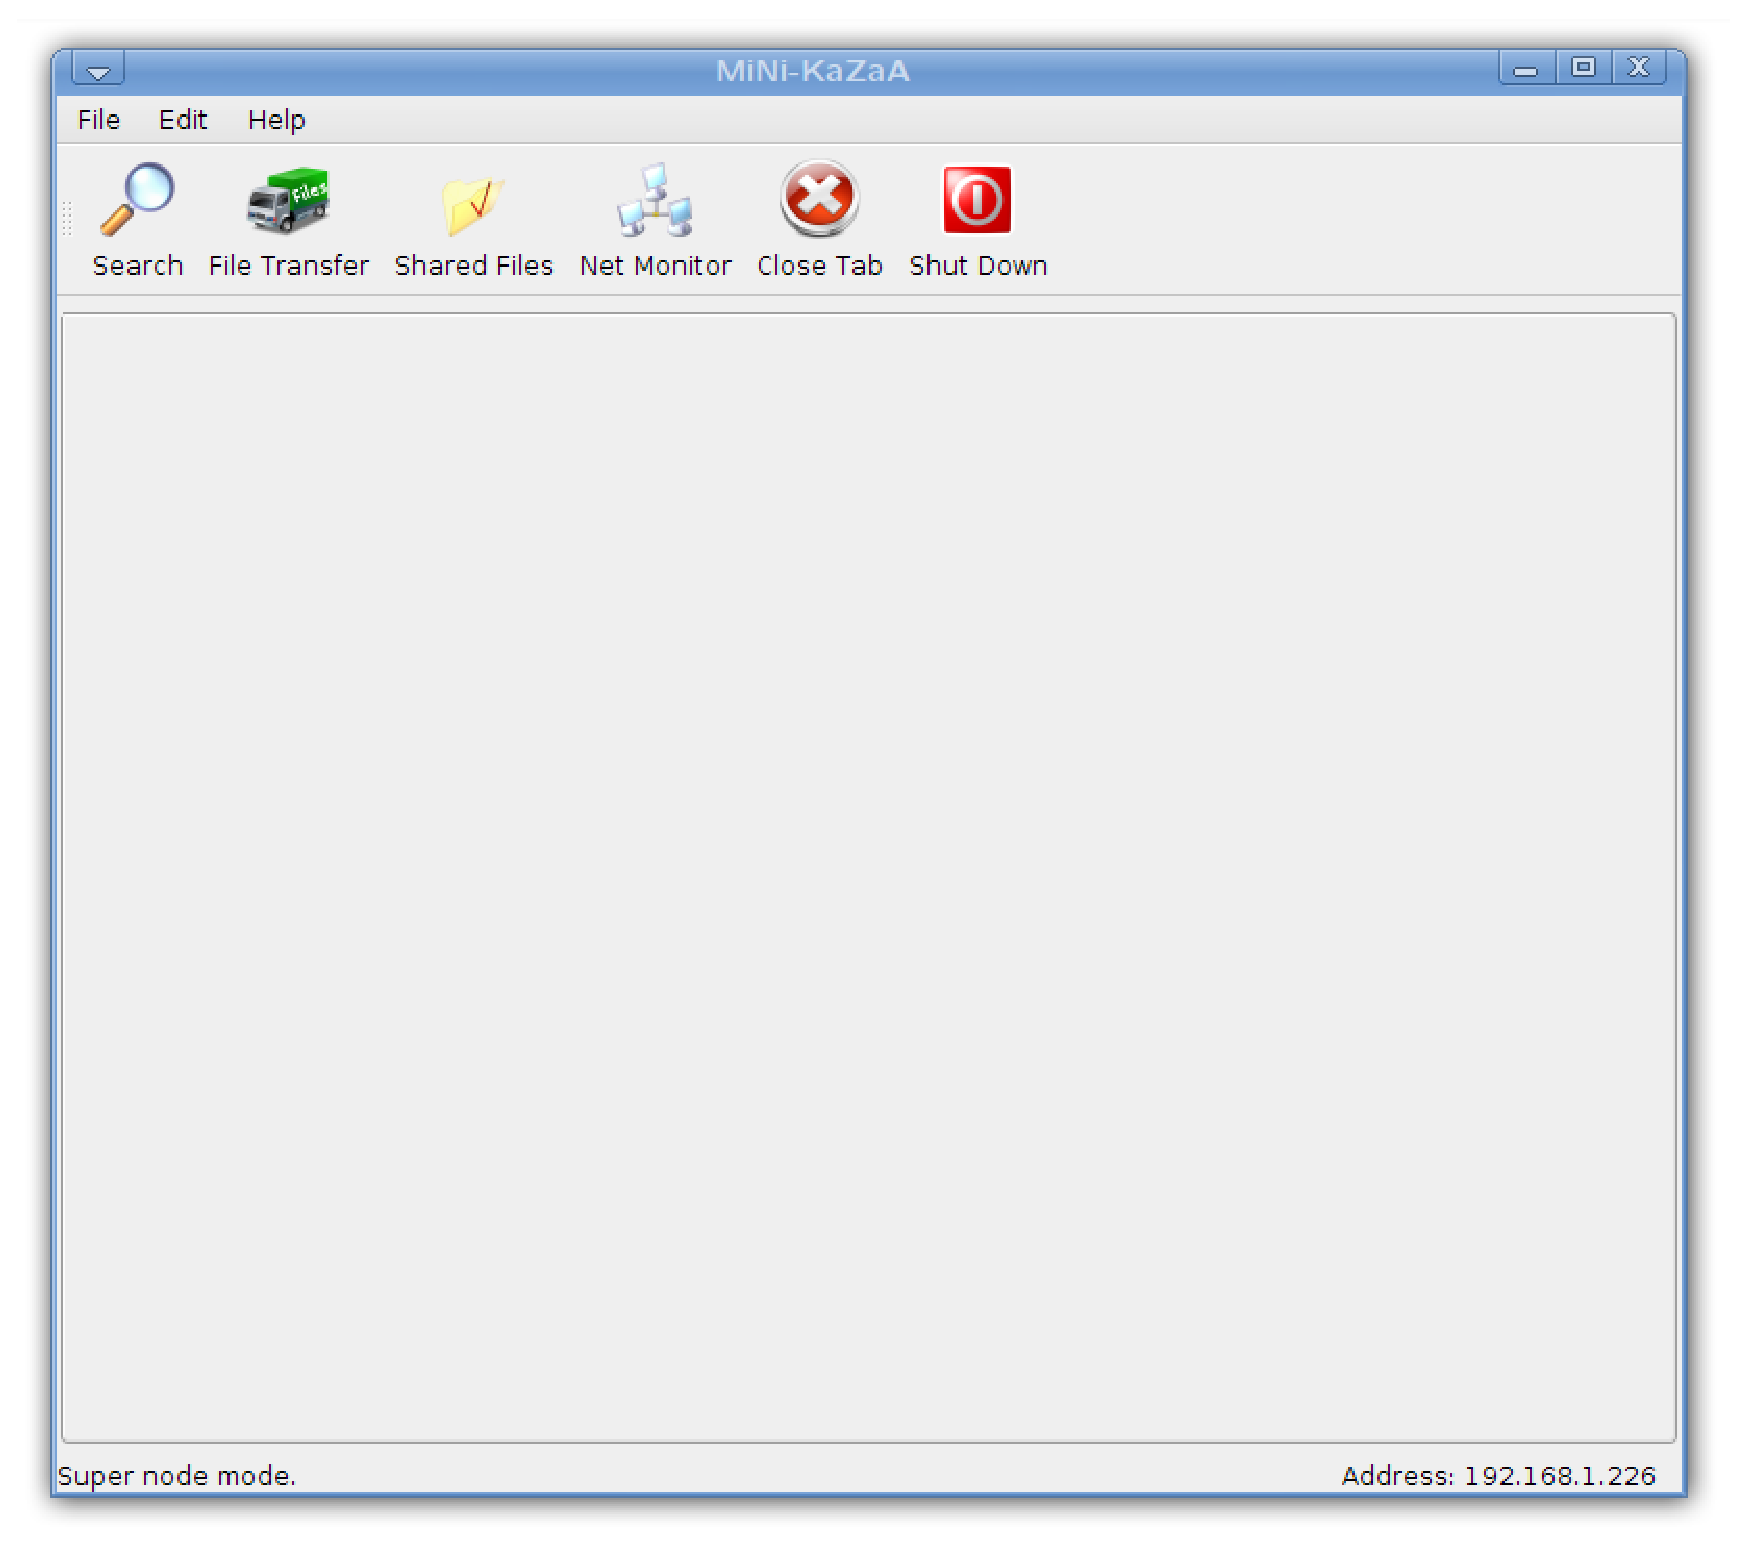
\includegraphics[width=250px,height=225px,bb=14 14 841 737]{images/mini_kazaa_client.eps}
 % mini_kazaa_client.eps: 0x0 pixel, 300dpi, 0.00x0.00 cm, bb=14 14 841 737
 \caption{L'interfaccia grafica principale del client.}
 \label{fig:mini_kazaa_client}
\end{figure}


%Spiegazione implementazione delle peculiarità dell'ordinary node
\chapter{Ordinary Node}
\section{Le classi del package ordinarynode}
All'interno del progetto Mini-KaZaA ogni package contiene delle classi che sono state scritte non solo per il tipo di nodo specifico, ma che, grazie alla \emph{modularità} e alla \emph{genericità} dei metodi, sono utili a tutti i tipi di nodi.
Di seguito quindi presentiamo le varie classi del package ordinarynode, ma non vanno pensate come dedicate esclusivamente al tipo di nodo ON. Vanno piuttosto legate agli ON da un punto di vista concettuale, ma nulla vieta di utilizzare queste pratiche classi nei SN.

\subsection{OrdinarynodeFiles.java}\label{sec:on_files}
La classe \verb|OrdinarynodeFiles.java| si occupa di indicizzare i file che il client decide di condividere all'interno della rete.
%\ref{sec:mk_filedescriptor}.
Questa classe implementa \emph{Observable}, quindi è sempre possibile monitorare tutte le informazioni sui file condivisi nella rete da parte del client.
Per essere utilizzata il più possibile, la classe utilizza gli attributi che sono descritti, assieme al costruttore della classe, nel seguente frammento di codice.
\begin{lstlisting}
private ArrayList<MKFileDescriptor> file_list;
private NodeInfo my_info;

public OrdinarynodeFiles(NodeInfo infos) {
	this.my_info = infos;
	this.file_list = new ArrayList();
}
\end{lstlisting}

L'\emph{ArrayList} di \emph{MKFileDescriptor}(Sezione \ref{sec:mk_filedescriptor}), \verb|file_list| consente di contenere in memoria tutti i file che si è deciso di condividere tramite l'apposito form.
Fra gli attributi compare anche \verb|my_info| che viene utilizzato dal client per segnalare nella rete che un determinato \emph{set} di file appartiene a un certo nodo che ha come \emph{NodeInfo}, Sezione \ref{sec:nodeinfo}.

La classe predispone anche una serie di metodi che consentono di manipolare la lista di file per aggiungere, modificare, estrapolare le informazioni.

\subsubsection{addFiles}\label{sec:on_files_add}
\begin{lstlisting}
public synchronized void 
addFiles(MKFileDescriptor[] new_files) {
	for (int i = 0; i < new_files.length; i++) {

		if (!isIn(new_files[i])) {
			this.file_list.add(new_files[i]);
		}
	}
	this.setChanged();
	this.notifyObservers();
}
\end{lstlisting}
Questo metodo consente di inserire all'interno della lista un \emph{array} di \emph{MKFileDescriptor}.
La scelta di ricevere come parametro un array di \emph{MKFileDescriptor} è dettata da come Java interagisce con il file system.
Java, infatti, quando si effettua la selezione di un insieme di file dal file system, restituisce un array di \emph{File}.
\`{E} quindi più semplice, quindi preferibile, effettuare una conversione fra \emph{File} e \emph{MKFileDescriptor}.

\subsubsection{removeFiles}
\begin{lstlisting}
public synchronized void 
removeFiles(MKFileDescriptor[] old_files) {
        
	for (int i = 0; i < old_files.length; i++) {
		int index = 0;
		for (MKFileDescriptor file : this.file_list) {
			
			if ((old_files[i].
				getFileName().equals(file.
				getFileName())) &&
				old_files[i].getMd5().
					equals(file.getMd5()) &&
				old_files[i].getPath().
					equals(file.getPath())) {

				
				this.file_list.remove(index);
				break;
			}
			index ++;
		}

	}
	this.setChanged();
	this.notifyObservers();
}
\end{lstlisting}
Questo metodo consente di rimuovere un \emph{Array} di \emph{MKFileDescriptor} dalla lista di file condivisi. La scelta di avere come parametro
un array di \emph{MKFileDescriptor} è già stata spiegata in Sezione \ref{sec:on_files_add}.
\`{E} un metodo piuttosto semplice che scorre la lista di file e si interrompe quando il doppio controllo\footnote{Abbiamo inserito un doppio contorllo su md5 (Sezione \ref{sec:md5}) e sul path del file per evitare qualsiasi tipo di problema dovuto a malfunzionamenti o scritture di memoria eseguite in maniera scorretta.} su \emph{md5} e \emph{path} del file segnala che il file è stato individuato.
Una volta individuato il file, viene rimosso e il metodo viene interrotto.

\subsubsection{searchFiles}\label{sec:on_searchFiles}
\begin{lstlisting}
public synchronized 
ArrayList <OrdinarynodeFiles> 
searchFiles(String regex){

ArrayList <OrdinarynodeFiles> l = 
	new ArrayList();
	Pattern pattern = Pattern.compile(regex);
	OrdinarynodeFiles files_found = 
		new OrdinarynodeFiles(this.my_info);

	MKFileDescriptor [] new_array = null;
	for(MKFileDescriptor file : file_list){
		ArrayList <MKFileDescriptor> found_list = 
			new ArrayList();

			Matcher matcher = 
				pattern.matcher(file.getFileName());

			while(matcher.find()){
				found_list.add(file);
				new_array = 
					new MKFileDescriptor[found_list.size()];
				
				int index = 0;
				
				for(MKFileDescriptor file_just_found : found_list){
					new_array[index] = file_just_found;
					index ++;
				}
				
				files_found.addFiles(new_array);
				l.add(files_found);
			}

	}
	
	return l;
}
\end{lstlisting}
Questo metodo deve ritornare al chiamante un \emph{ArrayList} di \emph{Ordinarynode} in cui andranno inserite i risultati della ricerca.
 
La ricerca viene effettuata prendendo come parametro una stringa, \verb|regex|, che è un'espressione regolare.
Con questa espressione regolare il metodo invoca due diverse classi: \verb|Pattern|, che contiene tutti i pattern che l'espressione regolare contiene, \verb|Matcher|, che si occupa di controllare eventuali \emph{match}\footnote{Si ricerca una corrispondenza fra gli oggetti passati e i vari pattern dell'espressione regolare.} con i file della lista.
Una volta individuate delle corrispondenze, i file vengono inserite nella lista da ritornare, \verb|l|, assieme alle \emph{NodeInfo} relative al nodo proprietario dei file.
Infine viene fatto un \verb|return| della lista, anche se dovesse risultare vuota.
Ritornale comunque la lista anche se fosse vuota è stata una decisione presa per un' implementazione a noi piu' congeniale del progetto.
%scelta di progetto inviare anche risposte vuote

\subsection{OrdinarynodeDownloadMonitor.java}
Parliamo di una classe che serve per indicizzare tutti i download di una determinata sessione.
Questa classe implementa Observable, in modo che sia possibile far vedere in grafica in ogni momento lo stato dei download.

\verb|OrdinarynodeDownloadMonitor.java| ha un solo attributo che consiste in un \emph{ArrayList} di Download, Sezione \ref{sec:download_class}.
%Aggiungere un riferimento alla classe Download
Questo attributo nel costruttore viene inizializzato con un nuovo ArrayList, quindi ogni nodo che partirà avrà un suo \emph{DowloadMonitor}.
\begin{lstlisting}
ArrayList <Download> downloads;
    
public OrdinarynodeDownloadMonitor(){
	this.downloads = new ArrayList();
}
\end{lstlisting}

I file vengono divisi in parti come ved(remo) in Sezione \ref{sec:download_tcp}. A ogni parte ricevuta è quindi necessario andare ad aggiornare il numero di byte scaricati per quel file.
Questo è il compito del seguente metodo:
\begin{lstlisting}
public synchronized boolean addBytes(DownloadResponse part){
	//Individuo il download e agiungo i byte
	for(Download d : downloads){
		if(d.getFile().
				getMd5().
				equals(part.getFile())){
			d.updateDownloadBytes(
				part.getPart().length);
			
		}
	}

	//Notifico il cambiamento
	this.setChanged();
	this.notifyObservers();

	return true;
}
\end{lstlisting}

Questo metodo, quindi richiama l'attenzione di tutti gli \emph{Observer} per aggiornare lo stato dei download.
Infine, i metodi \verb|set| e \verb|get| sono piuttosto semplici e non meritano particolare attenzione.

\subsection{OrdinarynodeFoundList.java}
La classe \verb|OrdinarynodeFoundList.java| consente di enumerare molto facilmente i risultati delle ricerche che si sono effettuate.
Si compone dei seguenti attributi:
\begin{lstlisting}
private int id;
private ArrayList<SearchField> found;

public OrdinarynodeFoundList(int n) {
	this.id = n;
	found = new ArrayList();
}
\end{lstlisting}
I due attributi descritti nel frammento di codice rendono molto semplice la gestione dei risultati delle ricerche.
\verb|int id| indica l' indice corrispondente alla query di ricerca che è stata lanciata.
\verb|ArrayList<SearchField> found| è una lista di tutti i risultati che corrispondono a una determinata ricerca, che vengono convertiti in oggetti di tipo \verb|SearchField|, Sezione \ref{sec:searchField_class}.
%Aggiungere riferimento in SearchFieldClass.java

I campi che costituiscono la lista \verb|found| vengono costruiti a partire dall' \emph{Answer} che arriva con indice corrispondente a \verb|id|.
Il frammento di codice che si occupa di inserire nella lista i campi correttamente costruiti è il seguente:
\begin{lstlisting}
public void add(Answer k) {
	ArrayList <OrdinarynodeFiles> list = 
		k.getFilesList();

	for(OrdinarynodeFiles of : list){
		ArrayList <MKFileDescriptor> 
			answer_files = of.getFileList();
			
		for(MKFileDescriptor files : answer_files){
			SearchField field = 
				new SearchField(files,of.getOwner());

			found.add(field);
		}
	}

	this.setChanged();
	this.notifyObservers();
}
\end{lstlisting}
Il metodo per prima cosa estrae la lista di \emph{OrdinarynodeFiles}, Sezione \ref{sec:on_files}, dopo di che scorre tutti gli \emph{OrdinarynodeFiles} ed estrae i vari descrittori di files, MKFileDescriptor \ref{sec:mk_filedescriptor}.
%Inserire un riferimento in MKFileDescriptor nel package util.

Il tipo \emph{MKFileDescriptor} però non consente un indicizzazione per proprietario, quindi, sempre per mantenere modularità nel codice, Mini-KaZaA converte i \emph{MKFileDescriptor} in \emph{SearchField} e li inserisce nell'\emph{ArrayList}.
Infine il metodo notifica tutti gli \emph{Observer} che stanno monitornando l'oggetto.

I vari metodi \verb|get| sono molto semplici, quindi non sono necessari ulteriori chiarimenti.

\subsection{OrdinarynodeQuestionList.java}
La classe \verb|OrdinarynodeQuestionList.java| consente di effettuare uno storage di tutte le ricerche che si stanno effettuando con il client Mini-KaZaA.

Questa classe ha solo un attributo, che è una \emph{List} di \emph{OrdinarynodeFoundList}.
\begin{lstlisting}
private List <OrdinarynodeFoundList> my_res_list;

public OrdinarynodeQuestionsList(){
	this.my_res_list = new ArrayList();
}
\end{lstlisting}

In \verb|my_res_list| vengono aggiunti di volta in volta i risultati delle varie ricerche.
Ogni volta che arriva il risultato di una ricerca sarà quindi necessario individuare a quale ricerca si riferisce.
Questo si può fare grazie all'indice \verb|id| che è contenuto sia nell'\emph{Answer} sia nella \emph{OrdinarynodeFoundList}.
\begin{lstlisting}
public synchronized void add(Answer a){
	for(OrdinarynodeFoundList l : this.my_res_list){
		if(a.getID() == l.getId()){
			l.add(a);
			return;
		}
	}
}
\end{lstlisting}
La classe \verb|OrdinarynodeQuestionList.java| mette anche a disposizione un metodo che consenta di individuare uno specifico file, tramite il codice md5, Sezione \ref{sec:md5}.
\begin{lstlisting}
public SearchField getFile(String md5){

	for(OrdinarynodeFoundList list : this.my_res_list){
		ArrayList <SearchField> file_list = 
			list.getFoundList();

		for(SearchField file : file_list){
			if((file.getFile().
				getMd5()).equals(md5)){
				
				return file;
			}
		}
	}

	return null;
}

\end{lstlisting}

\subsection{OrdinarynodeFriendRequest.java}\label{sec:friend_request}
La classe \verb|OrdinarynodeFriendRequest.java| è la classe su cui si basa l'\emph{overlay network} che si crea fra ON e SN.
Questa classe serve infatti per comunicare a un SN che l'ON, mittente della richiesta, ha scelto come SN di riferimento proprio lui.

\verb|OrdinarynodeFriendRequest.java| è un \emph{Java bean}, Sezione \ref{sec:java_bean}
%aggiungere un riferimento ai Java bean nel capitolo scelte di progetto.
che contiene solo i metodi \verb|set| e \verb|get| che si possono visualizzare nel seguente frammento di codice.
\begin{lstlisting}
private boolean want_to_be_friend;
private NodeInfo friend;

public OrdinarynodeFriendRequest(){ }
//Metodi set
public void 
setRelationship(boolean rel)
	{this.want_to_be_friend = rel;}

public void 
setInfo(NodeInfo info)
	{this.friend = info;}

//Metodi get
public boolean getRelationship()
	{return this.want_to_be_friend;}

public NodeInfo getInfo()
	{return this.friend;}
\end{lstlisting}

\section{Il cuore di un Ordinary Node}
Oltre a tutte le classi che sono state descritte nelle sezioni precedenti, un Ordinary Node ha anche un motore che combina tutte le classi in modo che siano realmente operative.
Come è possibile vedere il diagramma di disposizione logica di Mini-KaZaA, Sezione \ref{sec:UML_logica}
%creare un riferimento nella sezione UML
un Ordinary Node ha un motore principale e quattro interfacce principali con il mondo esterno:
\begin{itemize}
 \item \textbf{Grafica utente:}
che viene mostrata in modo chiaro e completo nel Capitolo \ref{chap:gui_package}, e nella Sezione \ref{sec:grafica};

 \item \textbf{Socket UDP:}
utilizzato solo per la misurazione delle latenze e mostrata nel Capitolo \ref{chap:scelte_di_progetto} in Sezione \ref{sec:ping};
 
 \item \textbf{Socket TCP:} 
utilizzato per la maggior parte delle comunicazioni nella rete, mostrato anch' esso nel Capitolo \ref{chap:scelte_di_progetto};

 \item \textbf{Comunicazioni RMI:}
utilizzato per l'interazione con il Bootstrap Server per gli aggiornamenti sui nodi della rete.
RMI che tratteremo nel dettaglio nel Capitolo \ref{chap:scelte_di_progetto}
\end{itemize}

Tutti questi componenti sono coordinati da un ``motore'' principale che ora andremo a descrivere.

\subsection{Engine}
Il motore di un Ordinary Node è il task 
\begin{verbatim}
public class OrdinarynodeEngine implements Runnable
\end{verbatim}
\verb|OrdinarynodeEngine| ha il compito di inizializzare le variabili e gli oggetti che poi utilizzaranno i \emph{thread} dell'ON e di far partire tutti i vari task che controllano le varie interfacce.

Guardiamo ora, in un piccolo frammento di codice, le variabili e gli oggetti istanziati dall'\emph{engine} dell'Ordinary Node.
\begin{lstlisting}
NodeInfo my_infos = new NodeInfo();

SupernodeList sn_list = new SupernodeList();

OrdinarynodeQuestionsList found_list = 
	new OrdinarynodeQuestionsList();
	
OrdinarynodeFiles my_file_list = 
	FileUtil.loadMySharedFiles(my_infos);
	
OrdinarynodeDownloadMonitor dl_monitor = 
	new OrdinarynodeDownloadMonitor();

BootstrapRMIWrapper rmi_stub = 
	new BootstrapRMIWrapper();
	
OrdinarynodeRefSn my_ref_sn = 
	new OrdinarynodeRefSn();
sn_list.addObserver((OrdinarynodeRefSn) my_ref_sn);

\end{lstlisting}

Fa quindi partire i \emph{thread} che possiamo vedere nel seguente listato.

\begin{lstlisting}
//Init TCP listener
OrdinarynodeTCPListener on_tcp = 
new OrdinarynodeTCPListener(
	this.my_conf, 
	found_list, 
	dl_monitor, 
	my_file_list);
Thread tcp_thread = new Thread(on_tcp);
tcp_thread.start();

//Init main GUI of supernode
MainGui main_gui = new MainGui(
		this.my_conf,
		my_file_list,
		found_list,
		sn_list,
		my_infos,
		dl_monitor,
		rmi_stub,
		my_ref_sn);
main_gui.setLocationRelativeTo(null);
main_gui.setVisible(true);

//Init RMI manager
OrdinarynodeRMIManager on_rmi = 
new OrdinarynodeRMIManager(
		this.my_conf,
		my_infos,
		sn_list,
		rmi_stub,
		my_ref_sn);
Thread rmi_thread = new Thread(on_rmi);
rmi_thread.start();

//Init ping service to receive pings
NodePong pong = new NodePong(this.my_conf);
Thread ping_service = new Thread(pong);
ping_service.start();
\end{lstlisting}
I \emph{thread} dei quali viene eseguito il comando \verb|.start()| sono quelli che poi andranno a gestire le varie interfacce che un client Mini-KaZaA deve avere.

\subsection{ON in ascolto sul socket TCP}
Ogni client Mini-KaZaA deve stare costantemente in ascolto sul socket TPC poichè da esso giungono la maggior parte delle comunicazioni.
Ogni client, pertanto, dedica un \emph{thread} alla funzione di ascolto su tale socket.

\verb|OrdinarynodeTCPListener.java| contiene un task con firma
\begin{verbatim}
public class OrdinarynodeTCPListener implements Runnable
\end{verbatim}

Questo task ha il compito di accettare le richieste che provengono dalla rete e creare un \emph{sotto-thread} che si occupi della richiesta specifica.
La classe \verb|OrdinarynodeTCPListener.java| ha i seguenti attributi.
\begin{lstlisting}
private NodeConfig my_conf;
private OrdinarynodeQuestionsList my_found_list;
private OrdinarynodeDownloadMonitor my_dl_monitor;
private OrdinarynodeFiles my_files;

public OrdinarynodeTCPListener(
		NodeConfig conf,
		OrdinarynodeQuestionsList list,
		OrdinarynodeDownloadMonitor dl_monitor,
		OrdinarynodeFiles files){

	this.my_conf = conf;
	this.my_found_list = list;
	this.my_dl_monitor = dl_monitor;
	this.my_files = files;
}
\end{lstlisting}
Gli attributi appena mostrati occorrono al \emph{TCPListener} per poterli poi far ereditare ai \emph{sotto-thread}. Essi poi li utilizzeranno per rispondere alle richieste che arrivano dalla rete.
Diamo uno sguardo al codice che si occupa di ricevere le richieste e far partire i \emph{sotto-thread}.
\begin{lstlisting}
ServerSocket listen_sock = null;
Socket incoming_sock = null;

ThreadPoolExecutor answer_pool = new ThreadPoolExecutor
		(10,15,50000L,
		TimeUnit.MILLISECONDS, 
		new LinkedBlockingQueue <Runnable>());

try{
	listen_sock = 
		new ServerSocket(this.my_conf.getPort());
}
catch(IOException ex){
	//Log
}

while(true){
	try {
		incoming_sock = listen_sock.accept();
		
		OrdinarynodeTCPWorkingThread tcp_job = 
				new OrdinarynodeTCPWorkingThread(
				incoming_sock,
				this.my_found_list,
				this.my_dl_monitor,
				this.my_files);

		answer_pool.execute(tcp_job);
	} catch (IOException ex) {
		//Log
	}
}
\end{lstlisting}
Il codice mostrato è piuttosto semplice ma utilizza una tecnologia Java molto utile: \emph{Thread Pool}\ref{sec:thread_pool}.
Ogni richiesta che il client riceve sul socket TCP viene infatti delegata a un \emph{sotto-thread} che la elabora, lasciando libero il thread principale di ricevere altre richieste sul socket.

\subsection{ON e RMI}
La connessione di un Ordinary Node al Bootstrap server avviene tramite protocollo RMI che consente di richiamare metodi di classi che stanno su una macchina remota e di elaborare i dati di ritorno.

La connessione tramite protocollo RMI viene gestita dal task
\begin{verbatim}
public class OrdinarynodeRMIManager implements Runnable
\end{verbatim}

Questa classe ha i parametri descritti nel frammento di codice che viene riportato sotto.
\begin{lstlisting}
private NodeConfig my_conf;
private NodeInfo my_infos;
private SupernodeList sn_list;
private BootstrapRMIWrapper rmi_stub;

public OrdinarynodeRMIManager(
		NodeConfig conf,
		NodeInfo info,
		SupernodeList list,
		BootstrapRMIWrapper rmi) {
		
	this.my_conf = conf;
	this.my_infos = info;
	this.sn_list = list;
	this.rmi_stub = rmi;
}
\end{lstlisting}
L'attributo \verb|my_conf| e \verb|my_infos| vengono utilizzati dalla classe per recuperare informazioni riguardanti il nodo come il tipo di nodo o l'indirizzo IP del nodo.
Gli attributi \verb|sn_list|, \verb|rmi_stub| e \verb|my_infos| vengono utilizzati all'interno di tutto il client ma vengono istanziati all'interno del task \verb|OrdinarynodeRMIManager| poichè le informazioni necessarie alla loro istanziazione sono recuperabili esclusivamente dal Bootstrap Server.

Diamo anche uno sguardo a come l'\emph{RMIManager} utilizza il protocollo RMI per recuperare le informazioni utili.
\begin{lstlisting}
Registry bootstrap_service;

BootStrapServerInterface callbacks_remote;

SupernodeCallbacksInterface callbacks_stub;

try {
	bootstrap_service = 
		LocateRegistry.getRegistry
		(my_conf.getBootStrapAddress(), 2008);

	//Divisione logica delle chiamate a procedure remote
	rmi_stub.setStub((BootStrapServerInterface) 
		bootstrap_service.lookup("BootStrap"));
		
	callbacks_remote = (BootStrapServerInterface) 
		bootstrap_service.lookup("BootStrap");

	ArrayList<NodeInfo> ni_list = 
		rmi_stub.getStub().getSuperNodeList();

	sn_list.refreshList(ni_list);

	//Managing callbacks.
	SupernodeCallbacksImpl callback_obj = 
		new SupernodeCallbacksImpl(
			this.sn_list, 
			this.my_conf);
			
	callbacks_stub = 
		(SupernodeCallbacksInterface) 
		UnicastRemoteObject.exportObject(callback_obj, 0);

	//Modifica degli attributi di NodeInfo
	try {
		my_infos.setInetAddress(
			InetAddress.getByName(my_conf.getMyAddress()));
			
		my_infos.setDoor(
			my_conf.getPort());
			
		my_infos.setCallbacksInterface(
			callbacks_stub);
			
		my_infos.setIsSn(
			my_conf.getIsSN());
			
		my_infos.setId(
			this.my_conf.getMyAddress()+
			":"+this.my_conf.getPort());
			
		this.my_sn_ref.setMyInfo(this.my_infos);
		
	} catch (UnknownHostException ex) {
		//Log
	}

	callbacks_remote.addOrdinaryNode(my_infos);

	sn_list.refreshList(ni_list);
	sn_list.refreshPing();

} catch (RemoteException ex) {
	//Error message
} catch (NotBoundException ex) {
	//Error message
}
\end{lstlisting}
Dal listato possiamo notare come in un primo momento l'\emph{RMIManager} si connette al Bootstrap Server tramite protocollo RMI e successivamente, una volta ottenute le informazioni riguardanti i SN presenti nella rete, inizializza tutti gli attributi della classe \emph{NodeInfo} poi richiama la procedura remota per aggiungere se stesso alla lista degli Ordinary Node presenti nella rete.

Le eccezioni catturate si riferiscono all'impossibilità di creare una connessione con il Bootstrap Server per errori nell'inserimento dell'indirizzo IP.
La gestione di tali eccezioni è stata oscurata per rendere più leggibile il codice.
In realtà viene presentato un \emph{Dialog Panel} che consente di modificare \emph{on the fly} l'indirizzo del Bootstrap Server.

\subsection{Scelta del SN al quale connettersi}\label{sec:scelta_sn}
%Parlare in particolare della classe OrdinarynodeRefSn.java
Un nodo di tipo ON che si connette alla rete ha bisogno di connettersi a un SN per poter accedere alla rete e cominciare a condividere ed effettuare ricerche all'interno della rete.
Scegliere però un nodo è uno dei problemi principali che un ON incontra appena inizia la sua attività.
Mini-KaZaA client ha quindi, grazie al paradigma \emph{Observer-Observable}, Sezione \ref{sec:obs-obs}, un sistema che monitora i SN nella rete
e sceglie il migliore.

Ciò avviene attraverso la classe \verb|OrdinarynodeRefSn.java| che contiene i senguenti attributi con il costurttore, descritti all'interno del
seguente frammento di codice.
\begin{lstlisting}
private Socket my_sn;
private NodeInfo best_sn;
private int num_query;
private ObjectOutputStream output_object;
private NodeInfo my_info;

public OrdinarynodeRefSn() {
	this.num_query = 0;
	this.my_sn = null;
	this.best_sn = null;
}
\end{lstlisting}
Gli attributi descritti sono quelli che servono per instanziare una connessione tra l'ON e il SN.
A fini statistici contiene anche il numero di query che vengono effettuate tramite questa connessione.
%Inserire questa parte nelle scelte di progetto.
Una prima domanda che potrebbe sorgere guardando questi attributi è: perchè creare un \emph{wrapper} per un socket?
La risposta sta nella dinamicità delle connessioni di rete che caratterizzano il progetto Mini-KaZaA.

Poichè è possibile che appena un ON entra nella rete non ci siano SN ai quali connettersi\footnote{La spiegazione al perchè è stato creato un \emph{wrapper} per un socket, Sezione \ref{sec:wrap_sock}.} Mini-KaZaA si affida ancora una volta al paradigma \emph{Observer-Observable}, Sezione \ref{sec:obs-obs}, per risolvere eventuali inconsistenze.

La firma della classe è
\begin{verbatim}
public class OrdinarynodeRefSn implements Observer
\end{verbatim}
quindi è interessante andare a vedere il metodo \verb|public synchronized| \verb|void| \verb|update(Observable o,| \verb|Object arg)| di cui la classe ha dovuto fare un \emph{override}.

\begin{lstlisting}
if (o instanceof SupernodeList) {
	SupernodeList list = (SupernodeList) o;

	if ((this.my_sn == null) && 
		(list.getList().size() > 0)) {
		
		NodeInfo best = list.getBest();

		this.setSocket(
			best.getIaNode(), 
			best.getDoor());
			
		this.best_sn = best;
		
		try {

			this.output_object = 
				new ObjectOutputStream(
					this.my_sn.getOutputStream());

			OrdinarynodeFriendRequest friend_request = 
				new OrdinarynodeFriendRequest();
				
			friend_request.setRelationship(true);
			
			friend_request.setInfo(my_info);
			
			output_object.writeObject(friend_request);

		} catch (IOException ex) {
			//Log
		}
	}
}
\end{lstlisting}
Innanzitutto il metodo verifica che l'oggetto che ha chiamato il metodo sia effettivamente di tipo \emph{SupernodeList} e 
quindi esegue un \emph{cast} per poterne sfruttare tutti i metodi.
Fondamentale è, quindi, l'istruzione \verb|NodeInfo best =| \verb|list.getBest();| che estrae dalla lista \verb|list| di tipo \emph{SupernodeList}
il nodo ``migliore''\footnote{Rimandiamo alla misurazione delle latenze, Sezione \ref{sec:ping}} e lo salva all'interno della variabile
\verb|best|.
Successivamente instanzia un \emph{stream} di dati verso il nodo \verb|best| e invia un oggetto di tipo \emph{OrdinarynodeFriendRequest}, Sezione
\ref{sec:friend_request}, con il valore \verb|true|, che indica l'inizio di un ``amicizia''.

Va fatto notare che con le istruzioni
\begin{lstlisting}
if ((this.my_sn == null) && 
		(list.getList().size() > 0)) {
\end{lstlisting}
l'ON evita di creare confusione nella rete istanziando più di una connessione.

%\subsection{Lo scambio di file}\label{sec:scambio}
%valutare la rimozione di questa subsection in favore di una subsection generale.
%eliminato e spostato in mini-kazaa client.tex

\subsection{Condivisione di file}%Valutarne la rimozione di questa subsection in favore di una subsection nella grafica
La condivisione di file avviene non appena l'utente di un ON decide di condividere file tramite l'apposito pannello descritto in Sezione \ref{sec:grafica}
Se si è un ON va però comunicata la selezione al proprio SN
%Spiegazione implementazione delle peculiarità del super node
\chapter{Super Node}
\section{L'interfaccia per le callback}
\section{Smistamento delle query}\label{sec:smistamento_delle_query}
%Descrizione package di utilità
\chapter{Il package Util}
\section{Calcolo dell'md5}\label{sec:md5}
%Una descrizione dettagliata del package contenente le classi 
%per la grafica
\chapter{Il package di grafica}\label{chap:gui_package}
\begin{figure}[t]
 \centering
 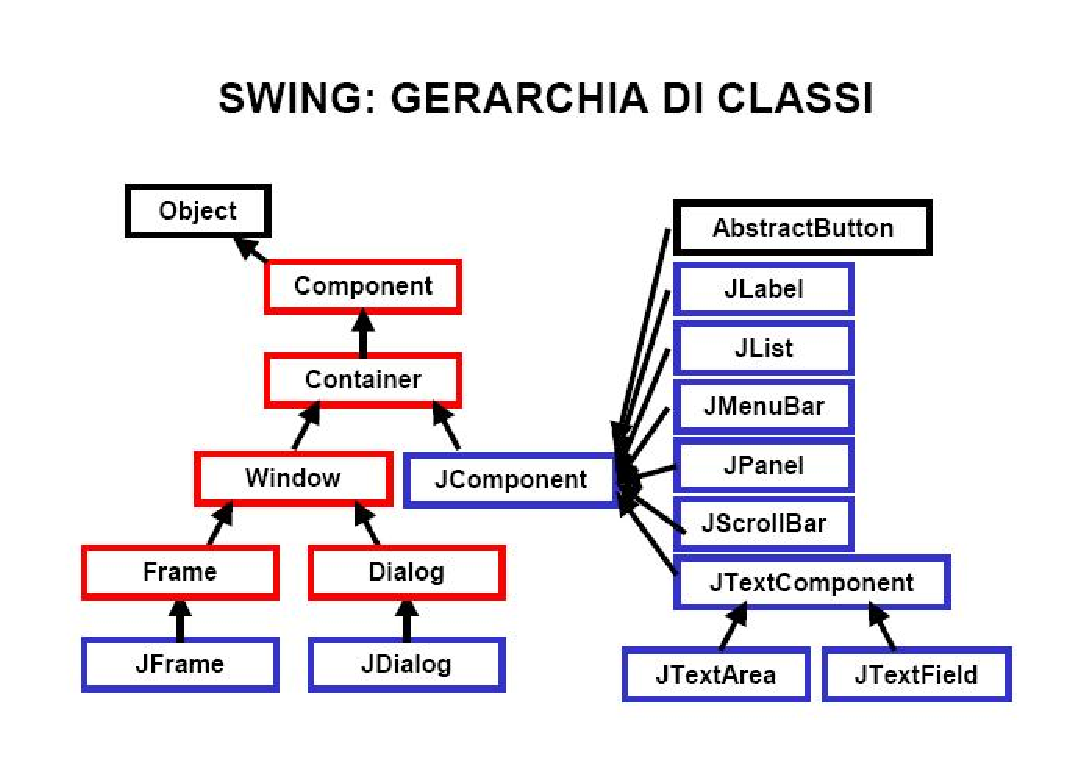
\includegraphics[width=350px,height=175px,bb=14 14 518 368]{images/swing_diagram.eps}
 % swing_diagram.eps: 0x0 pixel, 300dpi, 0.00x0.00 cm, bb=14 14 518 368
 \caption{La grafica con le librerie Swing.}
 \label{fig:swing_diagram}
\end{figure}

La parte grafica del MiniKazaa è stata implementata con la grafica che mette a disposizione il linguaggio Java e con l' ausilio dello strumento di programmazione NetBeans.
Nella parte che segue andiamo a vedere un pochino più di preciso cosa abbiamo usato per creare le interfaccie.

\section{Il campo di testo}
Il JTextField è un componente "campo di testo", usabile per scrivere e visualizzare una riga di testo.
Il campo di testo può essere editabile o no, il testo al suo interno è accessibile con getText() e modificabile con setText().
Ogni volta che il testo in esso contenuto cambia si genera un DocumentEvent nel documento che contiene il campo di testo.
Se invece è sufficiente registrare i cambiamenti solo quando si
preme INVIO, basta gestire semplicemente l' ActionEvent.

\section{I bottoni}
Quando viene premuto, un bottone genera un evento di classe ActionEvent.
Questo evento viene inviato dal sistema allo specifico ascoltatore degli eventi per quel bottone.
L'ascoltatore degli eventi deve implementare l' interfaccia ActionListener:
\begin{itemize}
\item può essere un oggetto di un'altra classe al di fuori del
pannello;
\item .. o può essere anche il pannello stesso nel quale (this).
\end{itemize}
Tale ascoltatore degli eventi deve implementare il metodo definito nella interfaccia actionListener void actionPerformed(ActionEvent ev);
che gestisce l'evento, nel senso che reagisce all'evento con opportune azioni.

\section{Gestore degli eventi}
Una volta generato l’oggetto evento, questo viene inviato ad un oggetto ascoltatore degli eventi (event listener).
L’event listener deve essere definito e creato da noi e deve essere associato al componente attivo, cosicché quando si genera un evento, la JVM sappia a chi inviare l’oggetto evento.
L’event listener gestisce l’evento mediante un opportuno metodo, che non è altro che l’implementazione di un particolare metodo di un’interfaccia associata a tali tipi
di eventi.


\section{Le tabelle di Java}
Una tabella è un componente che visualizza righe e colonne di dati. È possibile trascinare il cursore sui bordi delle colonne per ridimensionarle; è anche possibile trascinare una colonna in una nuova posizione. Le tabelle sono implementate dalla classe JTable.
Uno dei suoi costruttori è mostrato di seguito:
JTable(Object dati[][],Object intCol[])
dove dati è un array bidimensionale delle informazione da presentare e intCol è un array
monodimensionale con le intestazione delle colonne.
Ecco i passi per utilizzare una tabella in un frame:
\begin{itemize}
\item Creare un oggetto JTable
\item Creare un oggetto JScrollPane dove l'argomento del costruttore specifica la JTable appena creata. In questo modo la tabella verrà aggiunta al pannello
\item Aggiungere il pannello di scorrimento al pannello dei contenuti del JFrame (per intendere quello ottenuto tramite il metodo getContentPane()della classe)
\end{itemize}
Un JScrollPane è un pannello di scorrimento che presenta un'area rettangolare nella quale si può vedere un componente. Se il componente ha dimensione maggiore del pannello vengono fornite barre di scorrimento orizzontali e/o verticali.


\appendix
\chapter{Manuale d'uso}
Affrontiamo ora la parte piu' pratica del progetto.
\section{Installazione}
Anzitutto e' importante sapere che per poter utilizzare il prodotto da noi creato e' necessaria almeno una rete LAN o una rete INTERNET.
Un computer della rete deve fornire il servizio di bootstrap Server e quindi deve essere avviato come tale.
All'avvio del programma l' utente può decidere se essere un SuperNode o un OrdinaryNode.
Ricordiamo che questa decisione non sarà possibile modificarla nel seguito. 
A seconda della scelta appariranno a video le schermate da utilizzare ed il programma è pronto a funzionare.

\section{Come funziona}
Bene se siamo di fronte al programma correttamente installato ora non ci rimane che usarlo.
Se abbiamo deciso di essere SuperNode noi vogliamo oltre che poter cercare e scaricare sulla rete fornire il nostro servizio alla comunica globale.
Se abbiamo decido di essere OrdinaryNode noi vogliamo usufruire solamente del servizio di ricerca e download che offre Minikazaa.
	\subsection{Cercare e scaricare un file}
Per cercare e scaricare un file, è necessario inserire nella casella vuota il titolo del file che interessa trovare nella rete.
La nostra casella di ricerca interpreta la parola chiave inserita della casella come una $ *esempio* $ . Questo significa che tutti i file che contengono nel titolo la parola "esempio" verranno restituiti come canditati per lo scaricamento.
Nella tabellina sotto il campo dove è stata inserita la parola ora appariranno i riferimenti ai file che sono presenti sulla rete, i quali possono essere facilmente scaricati cliccando su comodo pulsate download
Il download che parte automaticamente è visibile e controllabile nella sezione chiamata FILETRANSFERT.

	\subsection{Aggiungere un file nella lista dei file condivisi}
Come tutti i servizi di file sharing minikazaa permette di aggiornare la lista dei file che è possibile scaricare.
Cliccando il bottone di Sharing viene caricato automaticamente un pannello che indica la lista dei file che sono stati messi in condivisione nella rete.
E' inoltre possibile aggiungere file alla lista cliccando su tasto add e rimuoverne altri cliccando sul tasto remove.

	\subsection{Controllare lo stato dei download}
Cliccando la sezione FileTranfert si apre un pannello che permette di controllare lo stato dei download dei file che desideriamo scaricare.
Nella tabella che si è appena aperta è possibile vedere il nome del file, la dimensione e il progressivo stato di scaricamento nella barra.
\subsection{Vita da OrdinaryNode}
	\subsection{NetMonitor}
Questo tasto risulta disabilitato se avete deciso di essere OrdinaryNode e invece è attivo se avete deciso di essere SuperNode.
Prendiamo ora il caso di essere SuperNode, e di avere aperto il pannello corrispondente a NetMonitor.
Nel suddetto pannello appare la situazione della rete al momento, piu' precisamente la lista dei SuperNode ai quali si è connessi.


	\subsection{Chiudere le schede}
I restanti tasti visibili nella schermata permettono di chiudere le schede aperte in precedenza.

	\section{Consigli degli autori per l' utilizzo}
Al fine di rendere un migliore servizio possibile diamo alcuni consigli per gli utilizzatori del nostro software.
Consigliamo quindi ad utilizzatori dotati di grosse quantità di file, ma soprattutto di grandi capacità di linea di offrire il loro servizio alla comunità globale e quindi di avviare l' applicazione come supernode.
Consigliamo invece agli utenti di piccole dimensione, che hanno difficolta ed un valore di upload limitato di preferire la modalità da ordinaryNode.
  

\end{document}
